\documentclass{article}
\newcommand{\beq}{\begin{equation}}
\newcommand{\eeq}{\end{equation}}
\newcommand{\ber}{\begin{eqnarray}}
\newcommand{\eer}{\end{eqnarray}}
\newcommand{\nn}{\nonumber}
\usepackage{graphicx}
\usepackage{amsmath}
\usepackage{amsfonts}
\usepackage{url}
\begin{document}
\title{Backward elimination}
\author{Nachiket Gokhale}
\date{\today}
\maketitle
\section{Introduction}
Given measured data {$\bf{y}\,\in\,\mathbb{R}^N$} and a feature vector {$\bf{x}$} we need to decide which of the features are really important. The algorithm to do this is given in the following figure from \url{https://towardsdatascience.com/backward-elimination-for-feature-selection-in-machine-learning-c6a3a8f8cef4}.
\begin{figure}
  \centering
  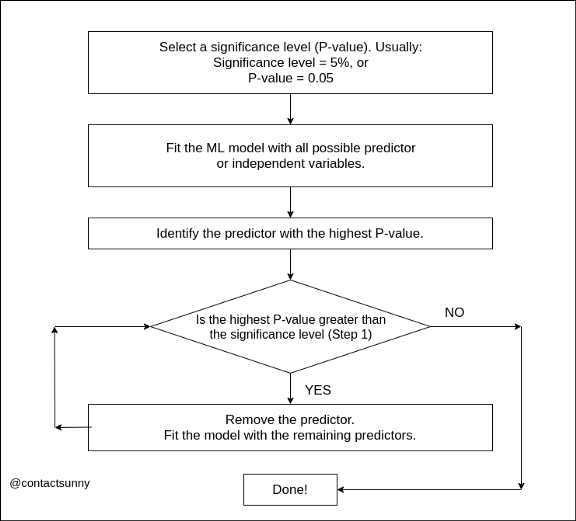
\includegraphics[totalheight=5cm]{images/backelim.png}
  \caption{Backward elimination from }
\end{figure}
Basically, the idea is to introduce the null hypothesis: there is no relationship between the output $y$ and the feature $x_ia$. In linear regression the form of the relationship is
\beq
y = \beta_0 + \beta_ix_i  \qquad \text{implied sum over } i
\eeq
The null hypothesis, that there is no relationship between $y$ and $x_i$, means $\beta_i=0$. The idea behind backward elimination is to compute the probability that $\beta_i=0$. If this probability (p-value) is less than significance level (SL) then we accept that $\beta_i$ is an important parameter in the model. p-value being less than SL means that there is a very small chance that the null hypothesis ($\beta_i = 0$) is true. (See: Elements of statistical learning Hastie, Tibshirani, Friedman: Pg 47,48). Let's assume Normal Distribution for the parameters $\beta_i$. We can estimate the variance by
\beq
\hat{\sigma}^2 = \frac{1}{N-p-1}\Sigma_{i=1}^{N}(y_i - \hat{y}_i)^2
\eeq
We can also say that
\beq
\hat{\beta} \sim N(\beta,(\bf{X}^T\bf{X}\sigma^2))
\eeq
where
\beq
\beta = E[\hat{\beta}|X]
\eeq
Also,
\beq
(N-p-1)\hat{\sigma}^2 \sim \sigma^2\chi^2_{N-p-1}
\eeq
Using Z scores we can estimate the probability that $\beta_j=0$ using $z_j$
\beq
z_j = \frac{\hat{\beta}}{\hat{\sigma}\sqrt{v_j}}
\eeq
Where $v_j$ is the $j^{th}$ diagonal element of $\bf{X}^T\bf{X}$.
\end{document}
